De Satellite heeft verschillende communicatiemiddelen, onder anderen ethernet en CAN Bus. Er zal gefocust worden op communicatie via CAN Bus aangezien dit het meest complex opgebouwd is.  De communicatie via CAN moet voldoen aan de volgende deelvraag: \textbf{Hoe kan er een robuuste communicatie gecreëerd worden tussen het hoofdsysteem en Satellite?} Er moet gekeken worden hoe dit stabiel en robuust gedaan kan worden.\newline


\noindent CAN is een groot onderdeel van de Sensor Maritime infrastructuur. De CAN-communicatie wordt gebruik om te kunnen communiceren met het hoofdsysteem. Hiervoor wordt een master en slave configuratie gebruikt. Het hoofdsysteem is de master en de Satellite en andere eindsystemen zullen dan de slave zijn. De master bepaalt hoe een slave apparaat zich gaat gedragen. CAN staat voor controlled area network, en maakt gebruik van een broadcast systeem. Dit betekent dat alle eindsystemen alle berichten ontvangen, De master kan niet specifiek naar een slave data sturen \autocite{can}. \newline

\noindent Sensor Maritime heeft een eigen protocol ontwikkeld wat gebouwd is op het CAN Bus protocol. Dit zal deels aangepast moeten worden om de Satellite sensoren te kunnen ondersteunen. Het huidige protocol is in afbeelding \ref{fig:canprotocol} te zien. Het protocol is opgebouwd uit velden wat uit 1 of 2 bytes bestaat. In tabel \ref{tab:cansensorprotocol} wordt beschreven wat de taak is van elk veld.
\begin{figure}[h!]
	\centering
	\label{fig:canprotocol}
	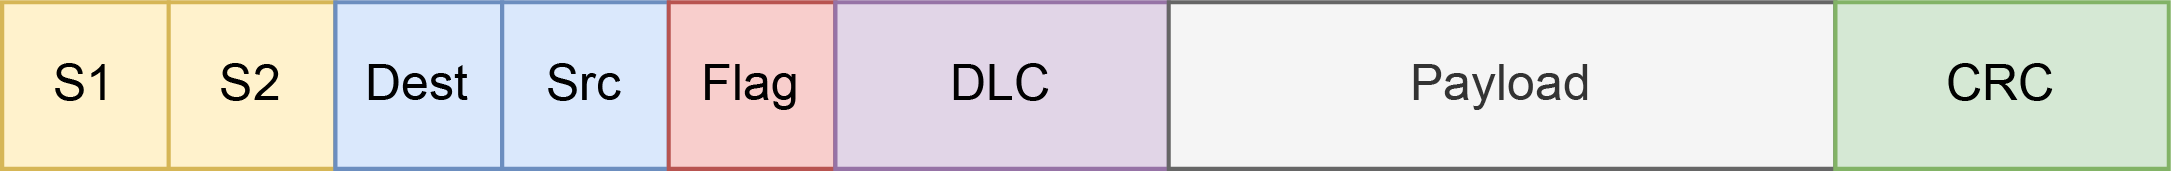
\includegraphics[width=0.75\linewidth]{voorstudie/communicatie/can.png}
	\caption{Sensor Maritime CAN protocol}
\end{figure}

\begin{table}[h!]
	\caption{Sensor Maritime CAN protocol opbouw}
	\label{tab:cansensorprotocol}
	\begin{tabular}{p{1.5cm}p{11.5cm}p{3cm}}
	\toprule
	\textbf{Blok} & \textbf{Beschrijving} & \textbf{Waarde}\\ \midrule
	S1		& De eerste start byte, dit geeft de start aan van het CAN bericht en wordt gebruikt voor herkenning, dit is een vaste waarde.	& 0x40 \\
	S2		& De tweede start byte, dit geeft de start aan van het CAN bericht en wordt gebruikt voor herkenning, dit is een vaste waarde. & 0x02 \\
	Dest	& Deze byte beschrijft voor wie het bericht bedoeld is.		& Verschillend per apparaat. \\
	Src		& Deze byte beschrijft van welke apparaat het bericht komt	& Verschillend per apparaat.\\ 
	Flag	& Dit geeft aan wat voor type bericht het is.             & 0 voor commando \\ 
			& & 1 voor request \\ 
	DLC		& DLC is een afkorting voor Data Length Code.             & \\ 
	Payload	& De data, dit verschillende aan de hand van de flag. & Verschillend per bericht\\
	CRC		& CRC staat voor Cyclic Redundancy Check, dit beschrijft hoe groot het bericht is wat verstuurd wordt. Hiermee kan de ontvanger valideren of het juiste is ontvangen. & Verschillend per bericht\\ \bottomrule
	\end{tabular}
\end{table}

\newpage
\subsection{Probleemstelling}
De huidige CAN BUS protocol ondersteunt de Satellite nog niet. De Satellite is een universeel systeem, waarmee verschillende sensoren verbonden zijn. Het huidige protocol is zo opgebouwd dat er maar één payload opgestuurd kan worden. Dit betekent dat als de Satellite twee sensoren op wil sturen het in de payload gestopt moet worden. Hiervoor moet een vaste structuur bepaald worden zodat de ontvanger weet wat er ontvangen wordt. Om dit probleem op te lossen zal er een aanpassing gemaakt moeten worden aan de bestaande CAN-protocol payload van Sensor Maritime. Hiervoor zijn verschillende oplossingen bedacht die hieronder worden beschreven. Uiteindelijk wordt toegelicht welke oplossing gekozen wordt en waarom. Voor alle payload structuren die beschreven worden zal er gebruik gemaakt worden van hetzelfde voorbeeld. Voor de voorbeelden worden er twee sensoren gebruikt die de Satellite zal ondersteunen. Deze twee sensoren zijn de inductie sensor en de altimeter sensor. De sensoren zullen gerepresenteerd worden als een getallen-lijst die begint bij 0. In het huidige systeem zijn er maar twee sensoren. Dit kan in de toekomst uitgebreid worden. Tabel \ref{tab:SensorRep} geeft een overzicht van de huidige sensoren en hun identificatie.

\begin{table}[h!]
	\centering
	\caption{Sensor identificatie representatie}
	\label{tab:SensorRep}
	\begin{tabular}{p{4cm}p{6cm}}
	\toprule
	Identificatie & Sensor        \\ \midrule
	0      & Inductor  \\
	1      & Altimeter \\ \bottomrule
	\end{tabular}%
\end{table}

\subsection{Structuur 1}
De eerste structuur is ontworpen om zo simpel mogelijk te zijn. Het idee bij dit ontwerp is dat er een identificatie is wat de sensor aangeeft en vervolgens gelijk de waarde van de sensor. Daarnaast voegt dit ook maar 1 byte toe aan de payload per sensor. Dit betekent dat het totale packet maar een aantal bytes groter zal zijn. De afbeelding \ref{fig:Structure1} geeft de opbouw en een voorbeeld weer, hierbij zijn twee sensoren te zien met de identificatie en de waarden van de sensor.
\begin{figure}[h!]
	\centering
	\label{fig:Structure1}


	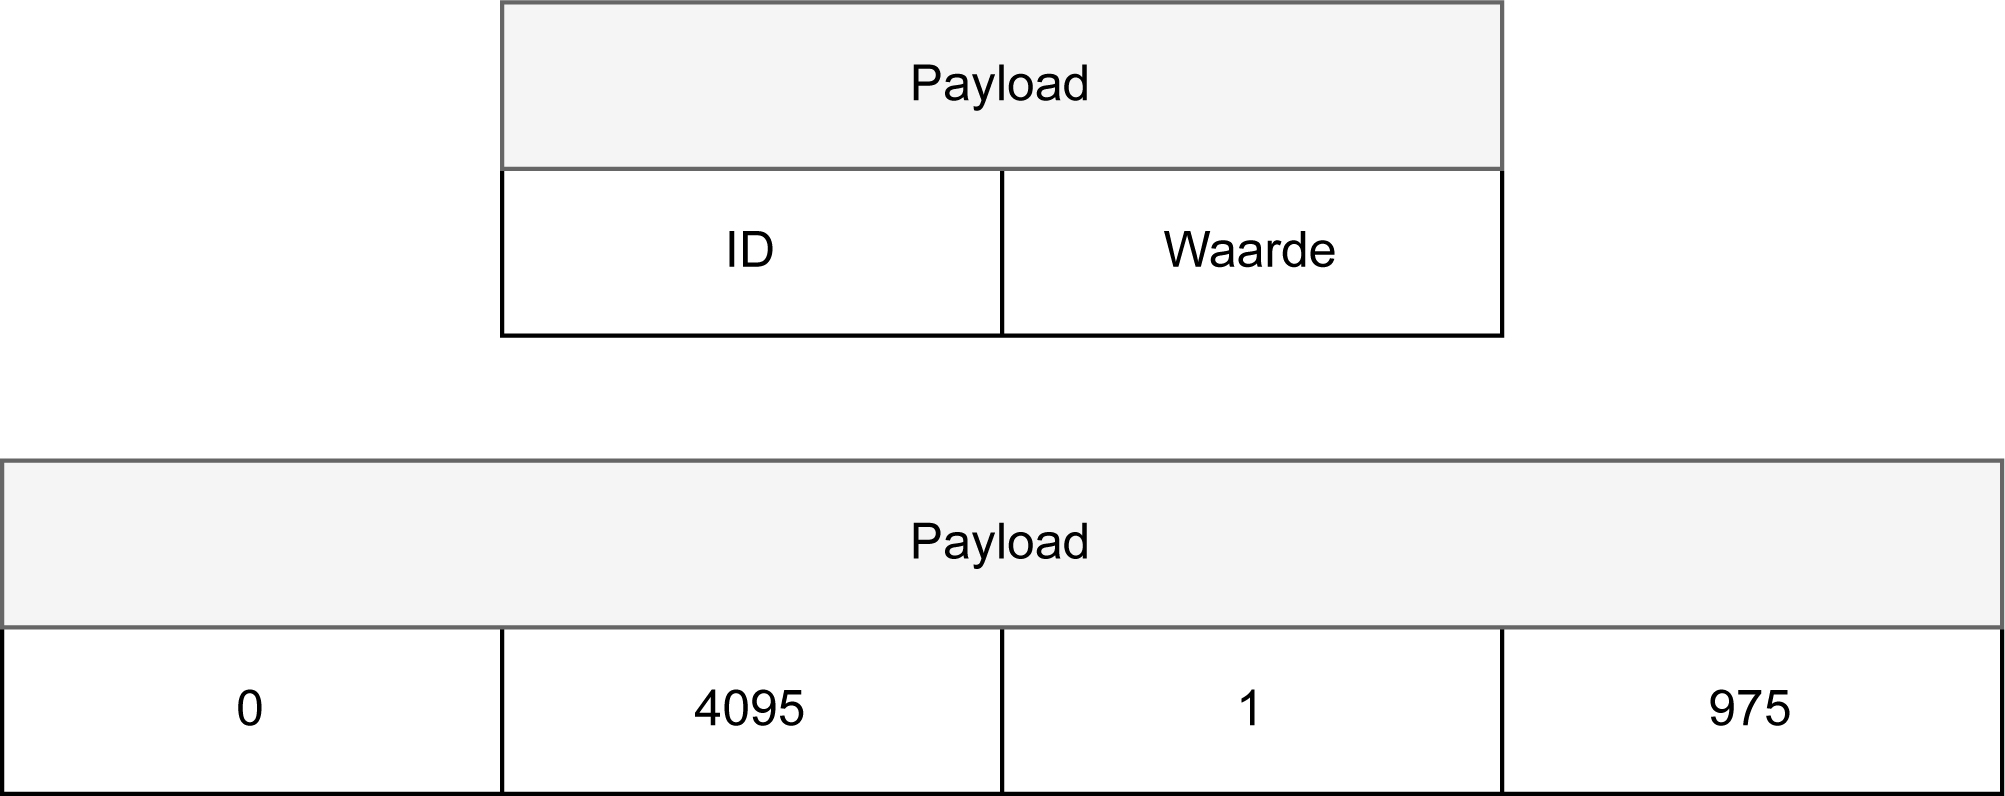
\includegraphics[width=0.75\linewidth]{voorstudie/communicatie/PayloadStructure1-01.jpg}
	\caption{Opbouw en voorbeeld van de payload structuur 1}
\end{figure}

\newpage
\subsection{Structuur 2}
Structuur 2 is opgezet om zoveel mogelijk te ondersteunen. Ten eerste ondersteunt dit meerdere datatypes, bijvoorbeeld 8, 16, 32 bit nummers maar ook 32 bit en 64 bit decimalen. Ten tweede geeft deze structuur duidelijk aan wat de grootte is van een packet. Packet grootte, geeft aan de hele sensor packet grootte in bytes. De identificatie geeft aan wat voor sensor het is. Dan komen er drie kolommen voor de waarde. Eerste wordt de waarde grootte in bytes gegeven, dan de waardetype en uiteindelijk de waarde zelf. In de volgende afbeelding \ref{fig:Structure2} is een overzicht te zien.
\begin{figure}[h!]
	\centering
	\label{fig:Structure2}

	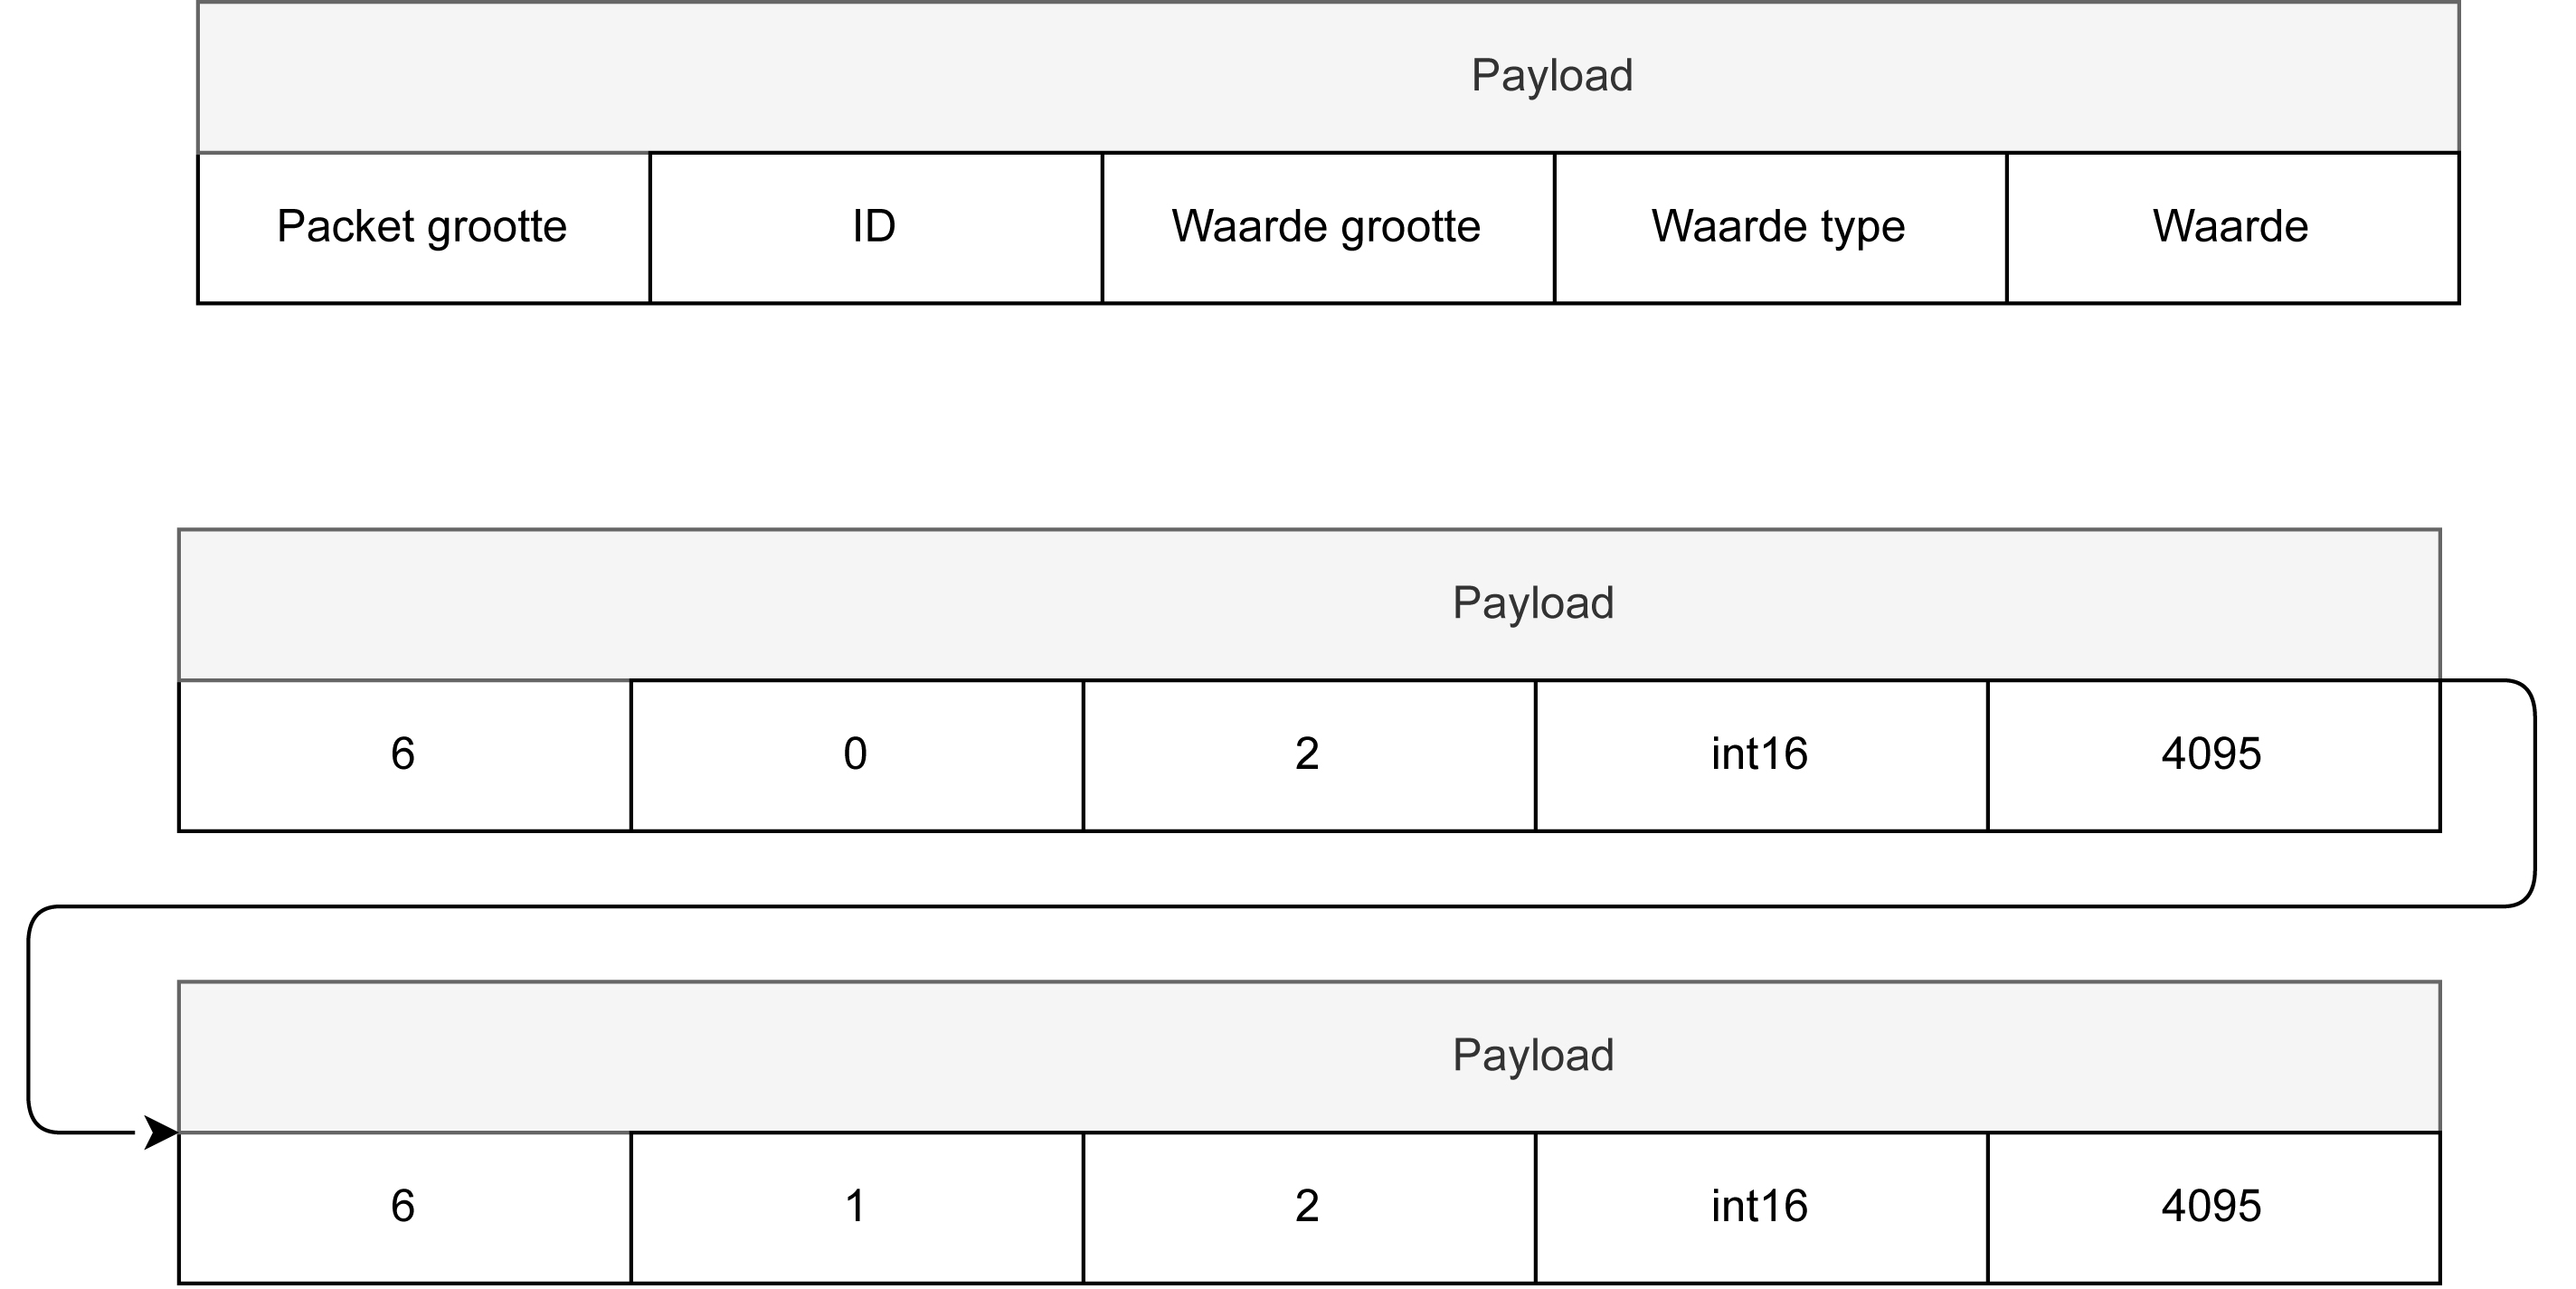
\includegraphics[width=0.75\linewidth]{voorstudie/communicatie/PayloadStructure2-01.jpg}
	\caption{Opbouw en voorbeeld van de payload structuur 2}
\end{figure}

\subsection{Structuur 3}
Dit is de laatste structuur die ontworpen is. Het is een combinatie van structuur 1 en structuur 2. Deze structuur heeft drie onderdelen voor een sensor. Als eerste zal de sensor identificatie meegegeven worden. Daarna komt de waarde grootte in bytes, en uiteindelijk wordt de waarde zelf gegeven. In afbeelding \ref{fig:Structure3} wordt de structuur en een voorbeeld weergeven.
\begin{figure}[h!]
	\label{fig:Structure3}

	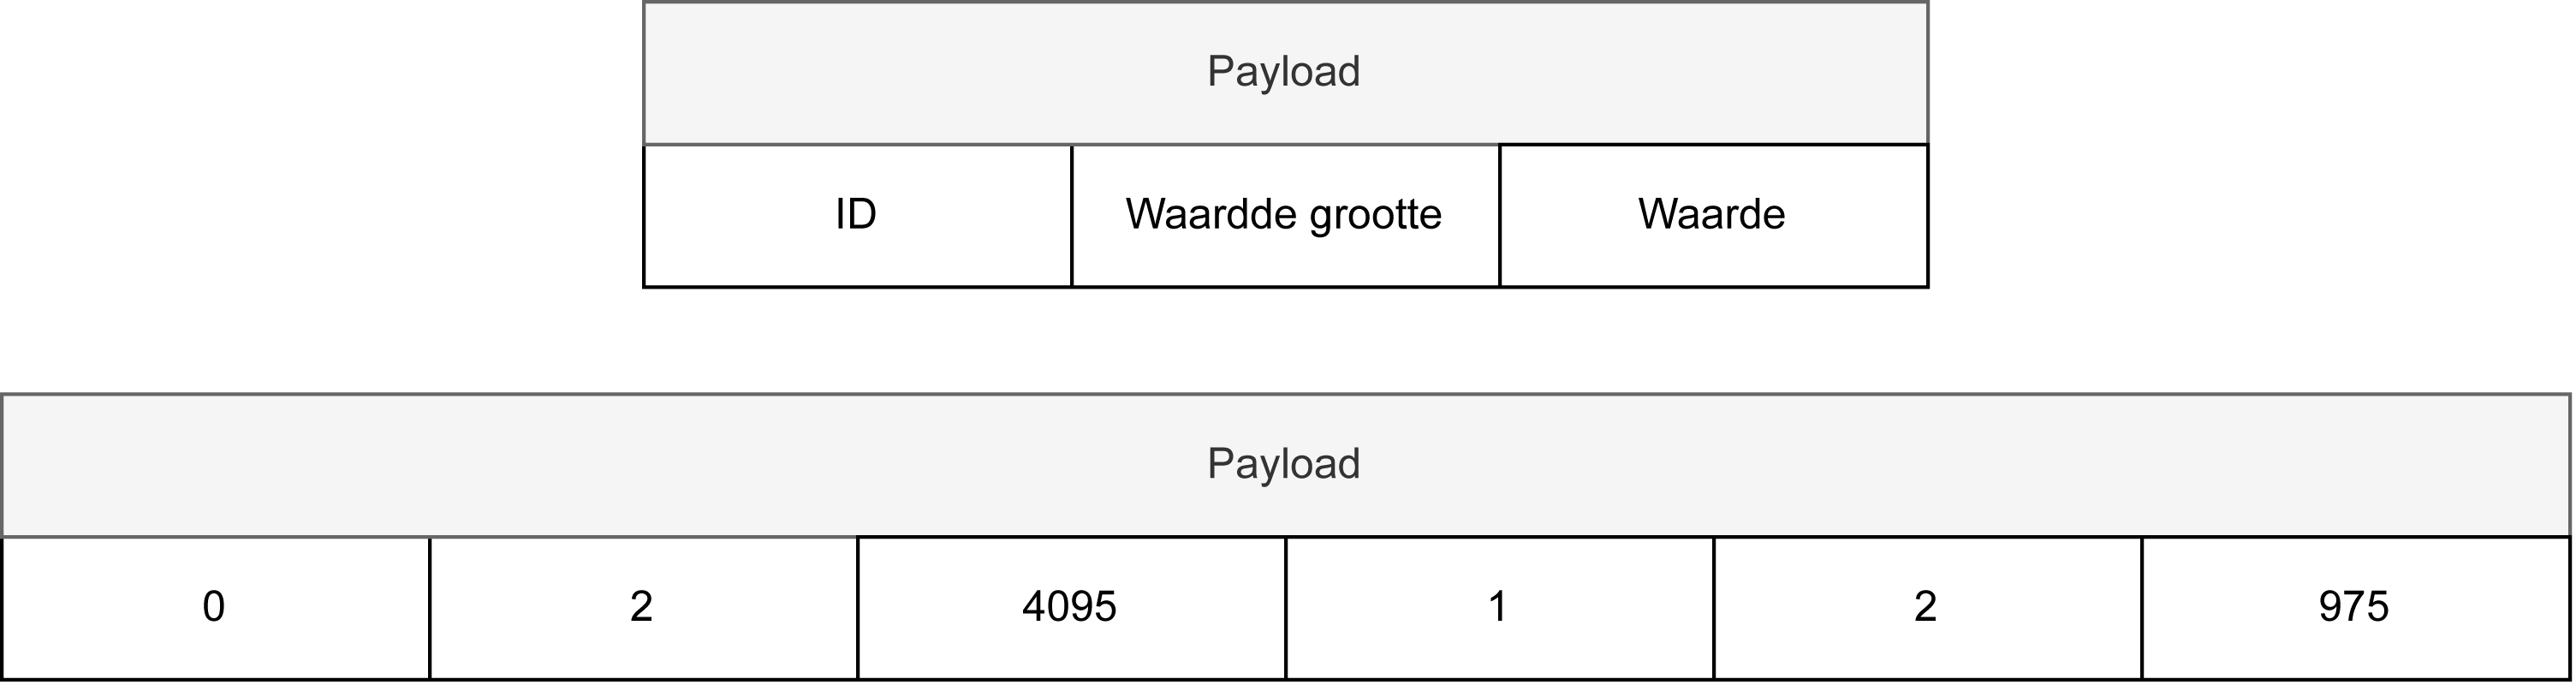
\includegraphics[width=\linewidth]{voorstudie/communicatie/PayloadStructure3-01.jpg}
	\caption{Opbouw en voorbeeld van de payload structuur 3}
\end{figure}

\newpage
\subsection{Communicatie flow}
Hieronder is in in figuur \ref{fig:comflow} te zien hoe de communicatie via CAN-bus gedaan wordt als er een bericht ontvangen wordt van het eindsysteem. Om een connectie te creëren zijn een aantal stappen nodig om dit goed af te handelen. Het hoofdsysteem kan verschillende type berichten sturen, in het vorige hoofdstuk is er vooral gefocust op de sensor payload structuur. Maar voor elk type bericht zal het apart afgehandeld worden. Er wordt dus eerst gecheckt wat voor type bericht het is, en daarvan splits het op in twee sectoren. De linker sector is een simpele structuur waarbij alleen wat data opgehaald of een karakter meegegeven moet worden. Bij de rechter sector wordt de payload structuur opgezet als eerste voor elke sensor dat de Satellite heeft. Dan wordt de payload berekend in bytes. Met de grootte in bytes kan het packet gemaakt worden. Vervolgens wordt het opgestuurd, dit zal een status code teruggeven. Als de communicatie al bezig is met iets versturen zal hierop gewacht moeten worden. Bij andere errors, failures zal een rood lichtje branden als status.
\begin{figure}[h!]
	\centering
	\label{fig:comflow}

	\includegraphics[width=0.7\linewidth]{ontwerp/communicatie/DataFlow.jpg}
	\caption{Activity diagram van de communicatie}
\end{figure}

\newpage
\subsection{Conclusie}
In dit subhoofdstuk is gekeken naar een manier om de huidige CAN Bus protocol zo aan te passen zodat het beter aansluit op de Satellite. De Satellite heeft verschillende sensoren die allemaal uiteindelijk in een payload moeten komen. Omdat het hoofdsysteem niet weet wat voor sensoren de Satellite op enig moment heeft, betekent het dat dit problemen kan veroorzaken. De nieuwe structuur voor de payload moet simpel te implementeren zijn, maar de payload moet ook niet veel groter worden. De eerste structuur is het simpelste maar is lastiger om te implementeren. Het grootste probleem is dat de buffer niet weet waar de volgende sensor begint. De waarde van sensor kan bijvoorbeeld 2 bytes zijn of 8 bytes. Het voordeel van structuur 1 is dat het een kleine structuur is waardoor de totale hoeveelheid data die opgestuurd wordt niet veel groter wordt. Structuur 2 is het tegenovergestelde van structuur 1, structuur 2 is makkelijk te implementeren omdat precies gezien kan worden wat verwacht kan worden per byte. Het probleem van structuur 2 is dat het veel groter is in bytes. Uiteindelijk is er nog structuur 3 en die zit tussen structuur 1 en 2, in vergelijking met hoe simpel het is om te implementeren en packet grootte. Een samenvatting van de structuren is te vinden in tabel \ref{tab:samenvattingstructuur}. \newline

\begin{table}[h!]
	\centering
	\caption{Samenvatting van CAN Payload structuren}
	\label{tab:samenvattingstructuur}
	\begin{tabular}{lll}
	\toprule
		Structuur nummer & Implementatie moeilijkheid & Packet grootte             \\ \midrule
		1                & Lastig                     & Klein (2 tot 9 bytes)      \\
		2                & Simpel                     & Groot (5 tot 12 bytes)     \\
		3                & Simpel                     & Gemiddeld (3 tot 10 bytes) \\ \bottomrule
	\end{tabular}%
\end{table}

\noindent In dit subhoofdstuk is er gekeken naar de volgende deelvraag \textbf{Hoe kan er een robuuste communicatie gecreëerd worden tussen het hoofdsysteem en Satellite?} Er is gekeken naar de moeilijkheid van de implementatie en de grootte van de payload. Deze twee onderdelen spelen een belangrijk onderdeel bij een robuuste communicatie. Daarom is er gekozen voor structuur 3, dit is een vrij simpele implementatie, en vergroot de payload maar weinig. Met deze payload-structuur weet het hoofdsysteem precies wat er gaat komen en hoeveel sensoren aan de Satellite verbonden zijn.